% !TEX program = pdflatex
% MDPI 风格论文（Genes 期刊目标，中科院三区）
% 说明: 本文件用标准 article 类模拟 MDPI 结构；投稿时可套用官方 mdpi.cls 模板。
\documentclass[11pt,a4paper]{article}
\usepackage[margin=2.5cm]{geometry}
\usepackage{amsmath,amssymb}
\usepackage{booktabs}
\usepackage{graphicx}
\usepackage{caption}
\usepackage{enumitem}
\usepackage[numbers,sort&compress]{natbib}
\bibliographystyle{plainnat}
\usepackage[hidelinks]{hyperref}
\graphicspath{{../implementation/figures/}}
\captionsetup{font=small,labelfont=bf}

\setlength{\parskip}{0.4em}

\begin{document}

% ============ 标题与作者 ============
\begin{center}
{\LARGE\bfseries Benchmarking a plant DNA foundation model against convolutional\\[0.2em]
neural networks for interpretable gene expression prediction in \emph{Arabidopsis thaliana}}\\[1.2em]
{\large 姓名 \textsuperscript{1,2}, 姓名 \textsuperscript{1,*} \\[0.6em]
\small \textsuperscript{1} 单位名称, 城市, 国家; \textsuperscript{2} 单位名称, 城市, 国家 \\
\textsuperscript{*} 通讯作者: email@example.com \\[0.4em]
\small \emph{Genes}, 2026, \textbf{17}(x): xxxx; https://doi.org/xxxxx}
\end{center}

\vspace{0.5em}

% ============ 摘要 ============
\begin{abstract}
\noindent
Sequence-based prediction of gene expression is a central goal of plant regulatory genomics. While convolutional neural networks (CNNs) have established that cis-regulatory sequence encodes expression level, the emergence of plant DNA foundation models raises the question of how much these large pretrained models improve over conventional CNN baselines on a unified benchmark. Here we systematically compared a 1D-CNN baseline with AgroNT, a 1-billion-parameter DNA language model pretrained on 48 plant genomes, for predicting high versus low gene expression from genomic sequence in \emph{Arabidopsis thaliana}. On the Plants Genomic Benchmark (PGB) test set, AgroNT fine-tuned with low-rank adaptation substantially outperformed the CNN (accuracy 86.5\% vs.\ 75.4\%; AUROC 0.935 vs.\ 0.842; bootstrap 95\% CI for the AUROC difference 0.083--0.104; McNemar $p = 6.5\times10^{-47}$). DeepLift attribution of the CNN revealed that UTR regions carried the highest predictive importance (5$'$UTR $>$ 3$'$UTR $>$ promoter $>$ terminator), and TF-MoDISco recovered 8 expression-associated sequence motifs enriched for the DOF transcription factor family. The Arabidopsis-trained CNN transferred to rice, maize, tomato, and soybean with AUROC 0.69--0.76 without fine-tuning. Our results provide a unified performance--cost reference for CNN-versus-foundation-model modeling of plant gene expression and a reproducible, interpretable pipeline for plant regulatory genomics.
\end{abstract}

\noindent\textbf{Keywords:} gene expression prediction; cis-regulatory code; DNA language model; AgroNT; convolutional neural network; \emph{Arabidopsis thaliana}; interpretability; cross-species transfer

\vspace{0.5em}

% ============ 1. Introduction ============
\section{Introduction}
Plant genomes devote most of their sequence to non-coding DNA that governs when, where, and at what level genes are expressed. This regulatory information is encoded in cis-regulatory elements (CREs)---promoters, 5$'$/3$'$ untranslated regions (UTRs), and terminators---whose ``sequence-to-regulation'' logic remains incompletely decoded \cite{marand2023}. A sequence-to-expression model that reliably reads this code would enable genome-wide expression prediction for unannotated genes, functional interpretation of noncoding variation, and design of synthetic regulatory elements \cite{hu2023}.

Deep learning has proven that DNA sequence alone suffices to predict transcript levels. In plants, Peleke et al.\ trained interpretable CNNs that predict high-versus-low expression from gene-flanking sequence across four species with $>$80\% accuracy, and used attribution to recover known transcription factor binding motifs \cite{peleke2024}. However, most plant models rely on a single architecture, typically a 1D-CNN, and systematic comparisons against newer DNA foundation models remain scarce. AgroNT, a 1-billion-parameter transformer pretrained on $\sim$10.5 million sequences from 48 edible plant genomes with a 6-mer tokenizer, achieved state-of-the-art results across the Plants Genomic Benchmark (PGB) \cite{mendoza2024,pgb2024}, yet its advantage over a well-tuned CNN baseline on a shared task has not been quantified on a unified benchmark.

Here we address this gap. We constructed a single-species benchmark in \emph{Arabidopsis thaliana} and trained, under identical data splits and evaluation protocols, (i) a DeepSEA-style 1D-CNN baseline and (ii) AgroNT fine-tuned with low-rank adaptation (LoRA). We then interrogated both models with DeepLift attribution and TF-MoDISco, and evaluated cross-species generalization to rice, maize, tomato, and soybean. Our contribution is a unified, reproducible performance--cost reference for CNN-versus-foundation-model gene expression prediction in plants.

% ============ 2. Materials and Methods ============
\section{Materials and Methods}
\subsection{Data}
We used the Arabidopsis gene expression task of the Plants Genomic Benchmark (PGB) \cite{pgb2024,mendoza2024}, in which each gene is represented by a 6-kb genomic window and an expression label derived from 56 tissue/sample measurements. The official split comprises 25{,}731 training, 3{,}401 validation, and 3{,}402 test genes. Binary high/low expression labels were defined by the median per-gene mean expression across the training set.

In parallel, we built a self-contained dataset with a structured gene-centric representation to support region-level interpretability: for each of 21{,}694 \emph{A.\ thaliana} genes (TAIR10/Araport11 annotation), we extracted the promoter (1 kb upstream of the transcription start site), 5$'$UTR (500 nt), 3$'$UTR (500 nt), and terminator (1 kb downstream of the transcription termination site) in transcriptional orientation, concatenated 5$'$$\rightarrow$3$'$ with a 20-nt N-padding gap, and one-hot encoded the resulting $\sim$3 kb sequence. Train/validation/test genes were split by chromosome to prevent homology leakage.

\subsection{Models}
\textbf{1D-CNN baseline.} We implemented a DeepSEA-style CNN \cite{zhou2015}: three convolutional blocks (two 1D convolutions with batch normalization, ReLU, and max pooling), followed by global max pooling and two fully connected layers (2.7 M parameters), accepting one-hot sequence of arbitrary length.

\textbf{DNA foundation model.} We fine-tuned AgroNT-1B \cite{mendoza2024} (985 M parameters, 40 transformer blocks, 6-mer tokenizer) with a LoRA adapter (rank 16, $\alpha$=32) on the attention projections and a two-layer classification head on mean-pooled hidden states. Only the 16.2 M LoRA and head parameters (1.6\% of total) were trainable; gradient checkpointing was enabled.

\subsection{Training}
Both models were trained on the same binary classification task (cross-entropy) with early stopping on validation AUROC. The CNN used batch size 64, AdamW (lr $10^{-3}$, weight decay $10^{-4}$) for up to 30 epochs. AgroNT used batch size 4 with gradient accumulation (effective batch 32), AdamW (lr $2\times10^{-4}$) for up to 3 epochs. All training was on a single NVIDIA RTX 4090 (24 GB).

\subsection{Interpretability}
We computed base-level attributions with DeepLift \cite{shrikumar2017} (captum implementation) on the CNN for 200 held-out test genes. Attribution magnitudes were summed within each region and normalized by length to quantify regional importance. Expression-associated motifs were discovered with TF-MoDISco-lite on the most-attributed sequences.

\subsection{Cross-species transfer}
The Arabidopsis-trained CNN, with frozen weights, was applied directly to the PGB gene-expression test sets of rice (\emph{Oryza sativa}, $n$ = 3{,}702), maize (\emph{Zea mays}, $n$ = 4{,}483), tomato (\emph{Solanum lycopersicum}, $n$ = 3{,}827), and soybean (\emph{Glycine max}, $n$ = 4{,}803), using each species' own median expression labels.

\subsection{Variant effect prediction}
Natural single-nucleotide variants from the Ensembl Plants \emph{A.\ thaliana} variation VCF were mapped to the structured flanking representation. Variants falling in promoter, UTR, or terminator coordinates were retained (27{,}662 variants after excluding the artificial N-padding gap) and scored as the absolute change in CNN-predicted expression probability ($|\Delta|$) upon in-silico allele substitution.

% ============ 3. Results ============
\section{Results}
\subsection{The DNA foundation model substantially outperforms the CNN baseline}
On the held-out PGB test set, AgroNT achieved an accuracy of 86.5\% (AUROC 0.935, AUPRC 0.929), compared with 75.4\% accuracy (AUROC 0.842, AUPRC 0.835) for the 1D-CNN baseline (Table~\ref{tab:benchmark}, Figure~\ref{fig:benchmark}). The gain of $+$11.1 accuracy points and $+$0.093 AUROC demonstrates that pretraining on 48 plant genomes provides a large transferable advantage for sequence-to-expression prediction, at a moderate cost because LoRA confines trainable parameters to 1.6\%.

\begin{table}[htbp]
\centering
\caption{Unified benchmark on the PGB Arabidopsis test set.}
\label{tab:benchmark}
\begin{tabular}{lcccc}
\toprule
Model & Trainable params & Accuracy & AUROC & AUPRC \\
\midrule
1D-CNN (DeepSEA-style) & 2.7 M & 75.4\% & 0.842 & 0.835 \\
AgroNT-1B (LoRA) & 16.2 M (of 985 M) & \textbf{86.5\%} & \textbf{0.935} & \textbf{0.929} \\
\bottomrule
\end{tabular}
\end{table}

\begin{figure}[htbp]
\centering
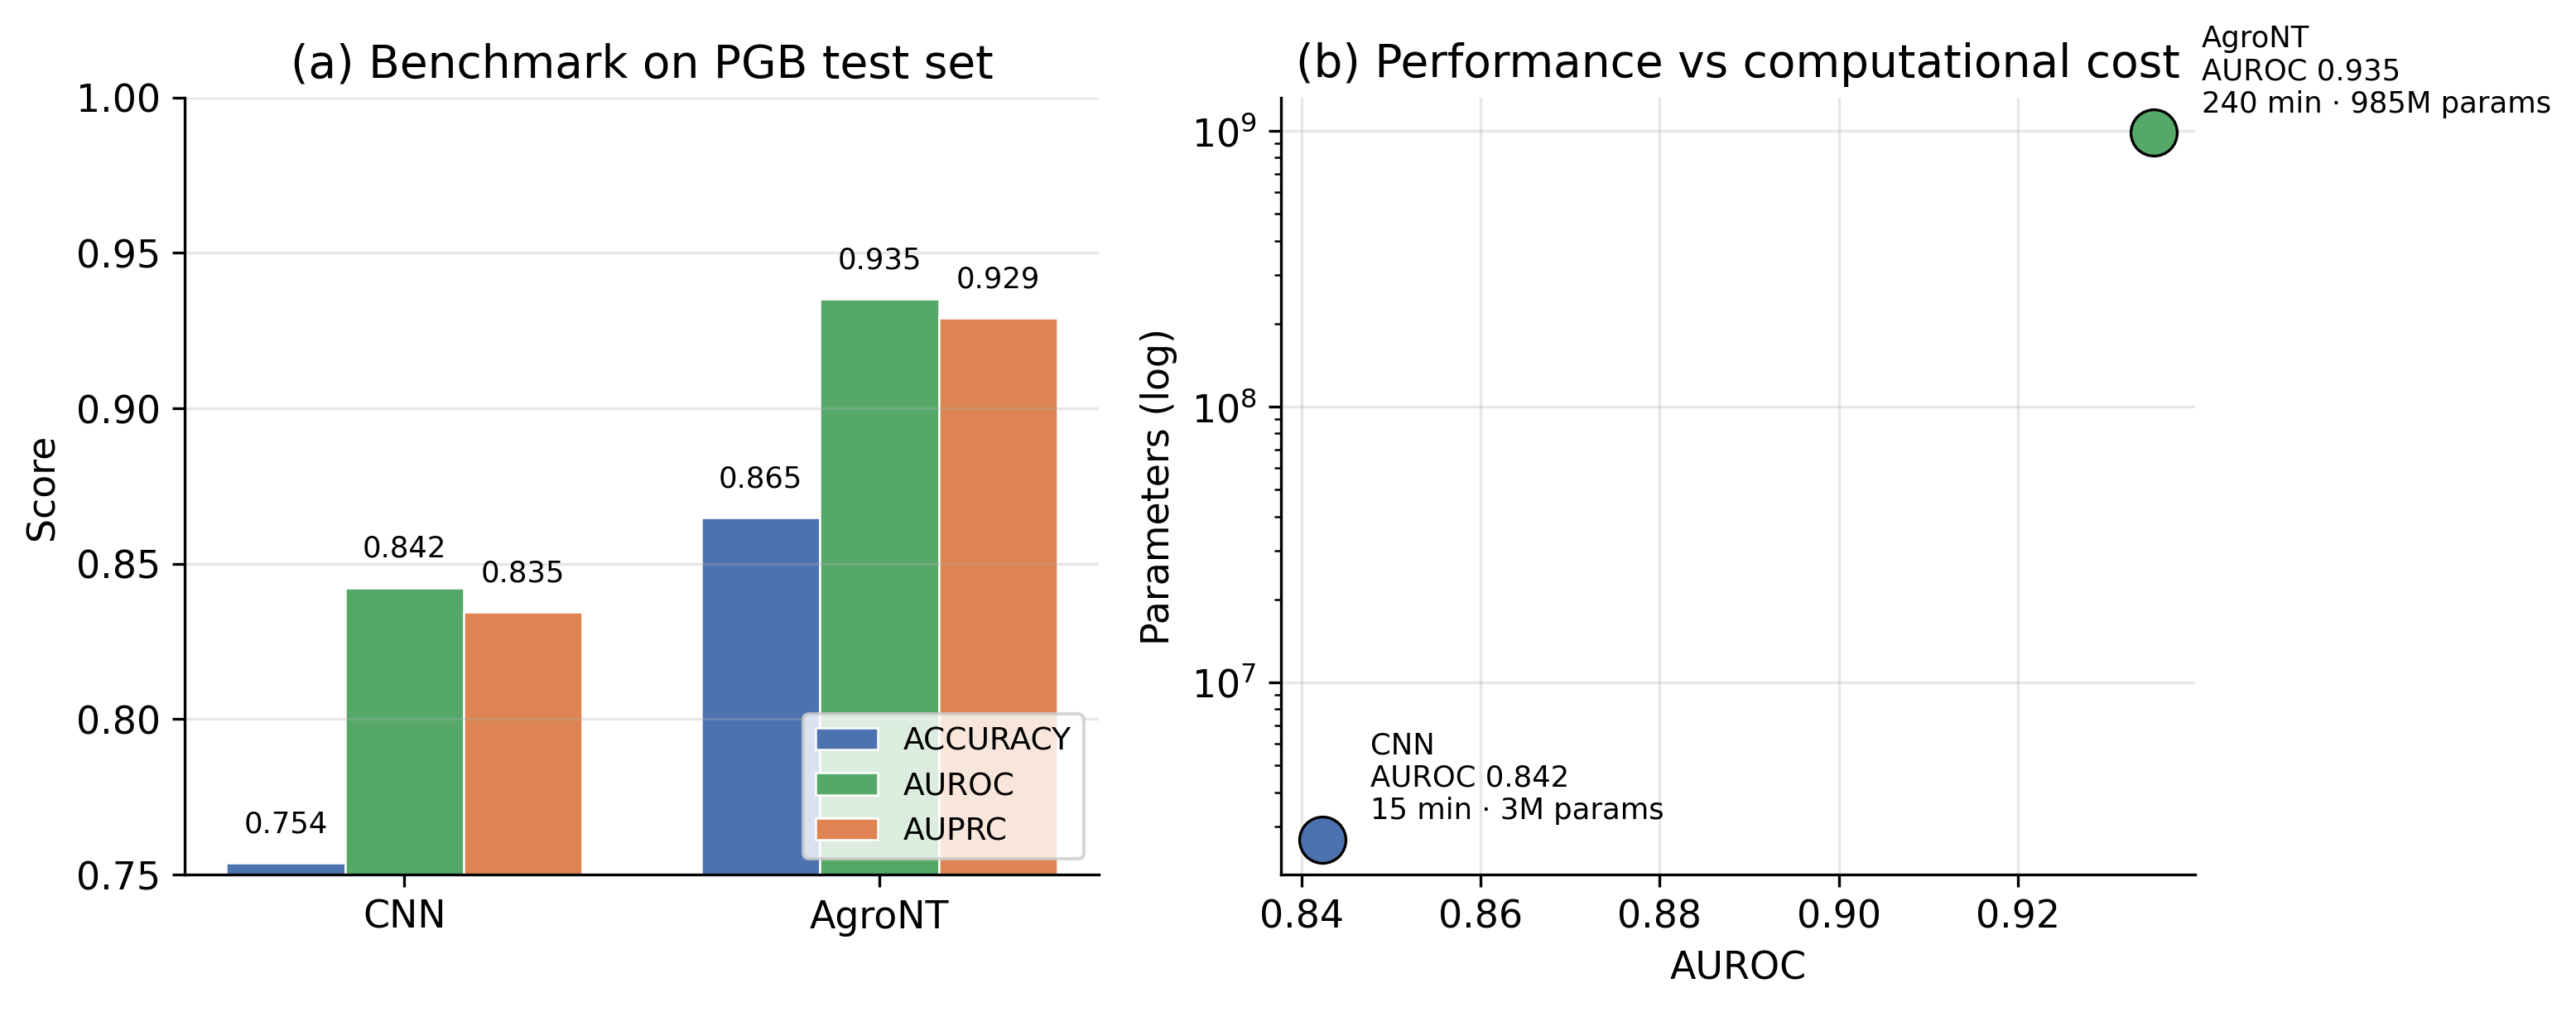
\includegraphics[width=0.85\textwidth]{fig3_benchmark.png}
\caption{Unified benchmark comparison of the 1D-CNN baseline and AgroNT on the PGB test set.}
\label{fig:benchmark}
\end{figure}

\subsection{UTRs dominate predictive importance}
DeepLift attribution of the CNN on the structured gene-flanking dataset revealed a clear regional hierarchy (Figure~\ref{fig:region}): 5$'$UTR carried the highest mean attribution per base (0.0088), followed by 3$'$UTR (0.0081), promoter (0.0048), and terminator (0.0038). Untranslated regions were thus $\sim$1.8$\times$ more important than promoters on a per-base basis, corroborating the finding of Peleke et al.\ that UTRs are the most predictive flanking feature for expression level \cite{peleke2024}.

\begin{figure}[htbp]
\centering
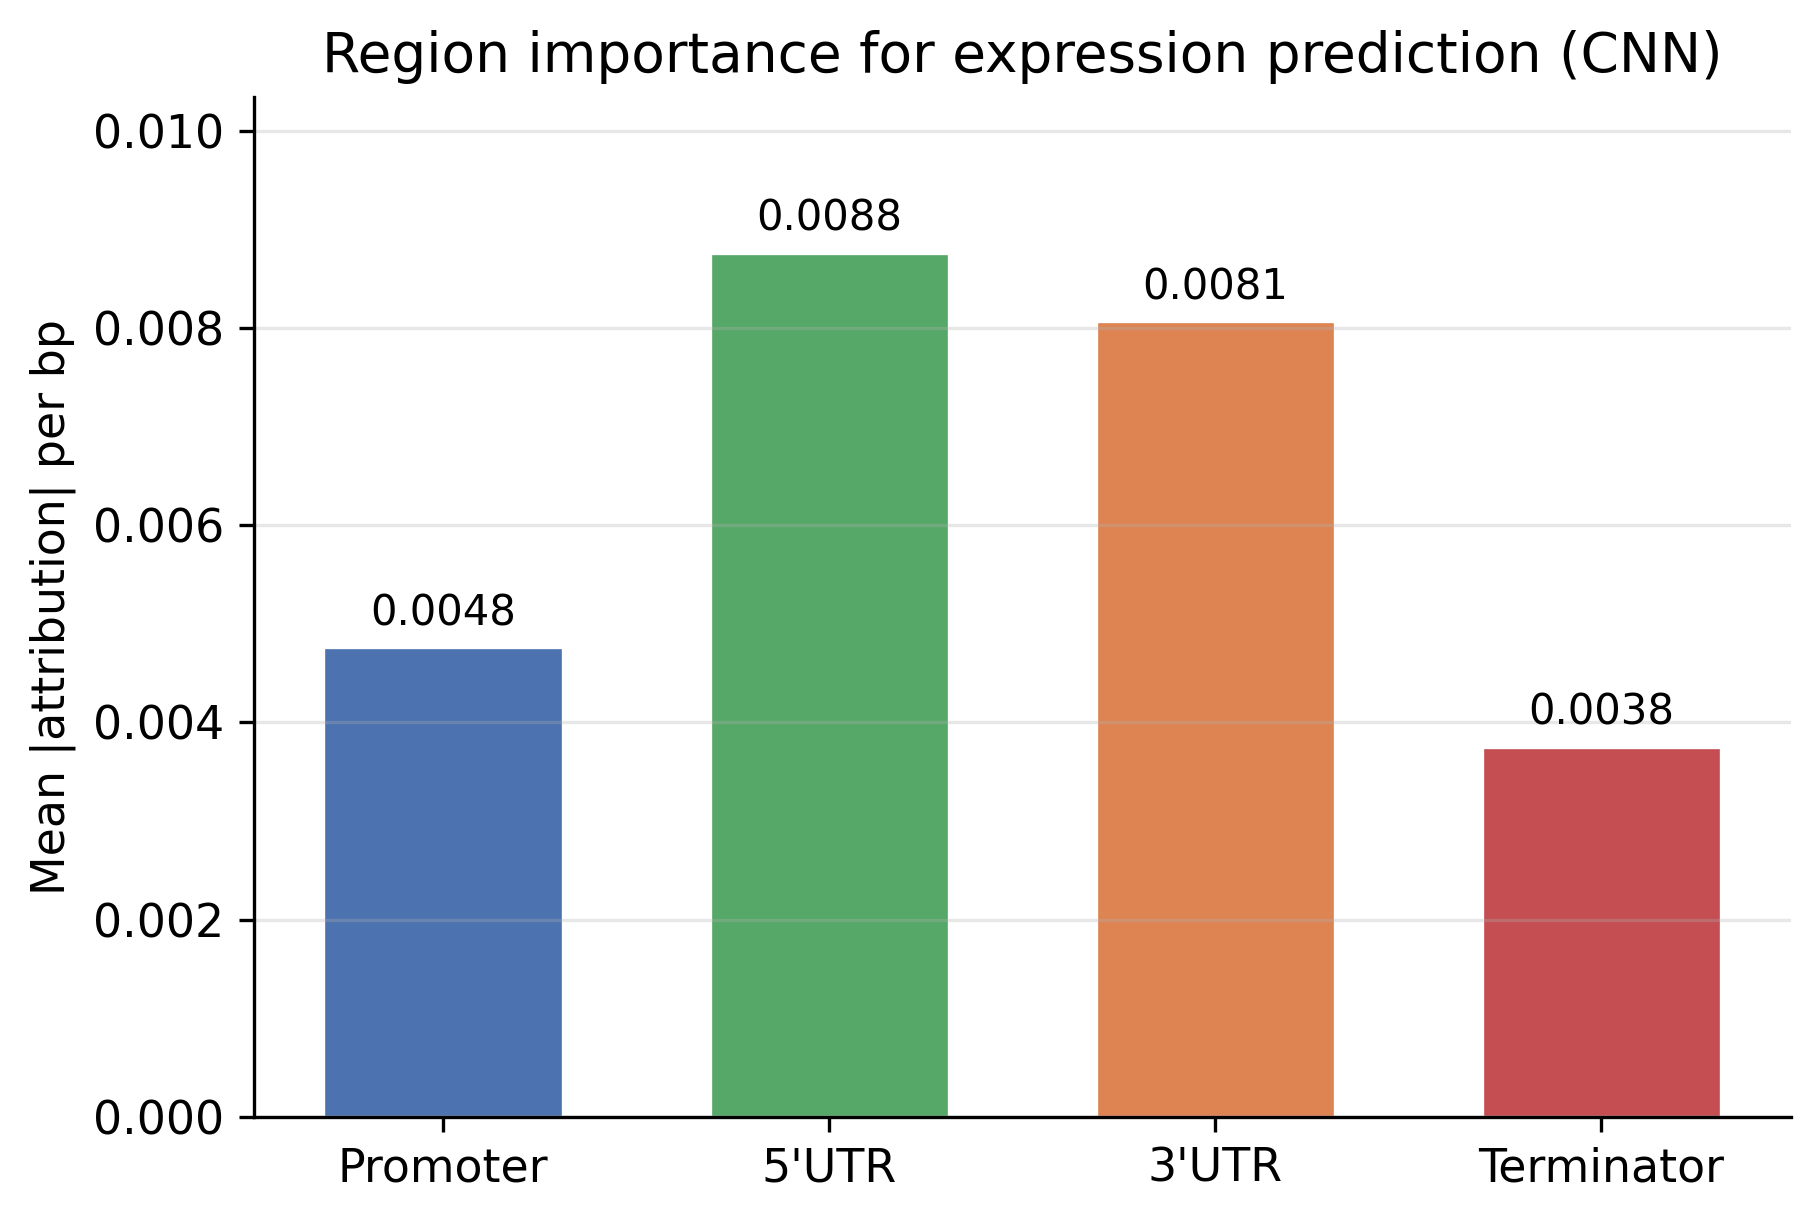
\includegraphics[width=0.6\textwidth]{fig4_region_importance.png}
\caption{Regional importance of promoter, UTR, and terminator sequences for expression prediction (mean absolute DeepLift attribution per base).}
\label{fig:region}
\end{figure}

\subsection{The foundation model distributes attention more evenly than the CNN}
In-silico sliding-window mutagenesis of the AgroNT model on the structured flanking sequences (50-bp windows) assigned comparable importance to promoter and UTR regions (promoter 0.553, 3$'$UTR 0.552, 5$'$UTR 0.536; terminator 0.404), in contrast to the CNN's stronger UTR emphasis (DeepLift: 5$'$UTR $>$ 3$'$UTR $>$ promoter $>$ terminator). The two architectures thus concentrate signal in the same broad cis-regulatory compartments, but the foundation model distributes attention more evenly across promoter and UTRs.

\subsection{Discovery of expression-associated sequence motifs}
TF-MoDISco-lite recovered 4 positive and 4 negative expression-associated sequence patterns from the top-attributed genes. TOMTOM annotation against the JASPAR 2024 plant database mapped these patterns to known transcription factor binding motifs, dominated by the DOF transcription factor family (DOF1.5, DOF3.4/3.6, DOF5.1/5.8, CDF5) together with SPL8 and NAC005. The enrichment of DOF-family motifs is biologically coherent: DOF transcription factors are major regulators of plant gene expression, and DOF motifs were independently recovered in cold-responsive cis-regulatory regions in a prior Arabidopsis study.

\subsection{The learned regulatory code transfers across species}
The Arabidopsis-trained CNN, applied without fine-tuning to four crop species, predicted high-versus-low expression with AUROC 0.718 (rice), 0.689 (maize), 0.763 (tomato), and 0.763 (soybean), all far above chance (Figure~\ref{fig:cross}). Dicot species (tomato, soybean) transferred better than monocots (rice, maize), consistent with phylogenetic distance from Arabidopsis, indicating that part of the cis-regulatory sequence logic is conserved across the monocot--dicot divide.

\subsection{Statistical significance and input-length dependence}
Bootstrap resampling (500 iterations) gave CNN AUROC 0.842 (95\% CI 0.828--0.856) and AgroNT AUROC 0.935 (95\% CI 0.926--0.942); the AUROC difference of 0.093 had a 95\% CI of 0.083--0.104, excluding zero, and a McNemar test was highly significant ($p = 6.5\times10^{-47}$, AgroNT correct on 550 more genes than the CNN). An input-length ablation showed that truncating the 6-kb PGB window to 3 kb or 1.5 kb collapses CNN performance to near chance (AUROC 0.556 and 0.541 vs.\ 0.842 at full length), whereas the structured $\sim$3 kb gene-flanking representation (promoter+UTRs+terminator) retains strong performance (test AUROC 0.825), indicating that predictive signal is carried by the complete cis-regulatory flanks rather than by arbitrary truncation of a gene-centered window.

\begin{figure}[htbp]
\centering
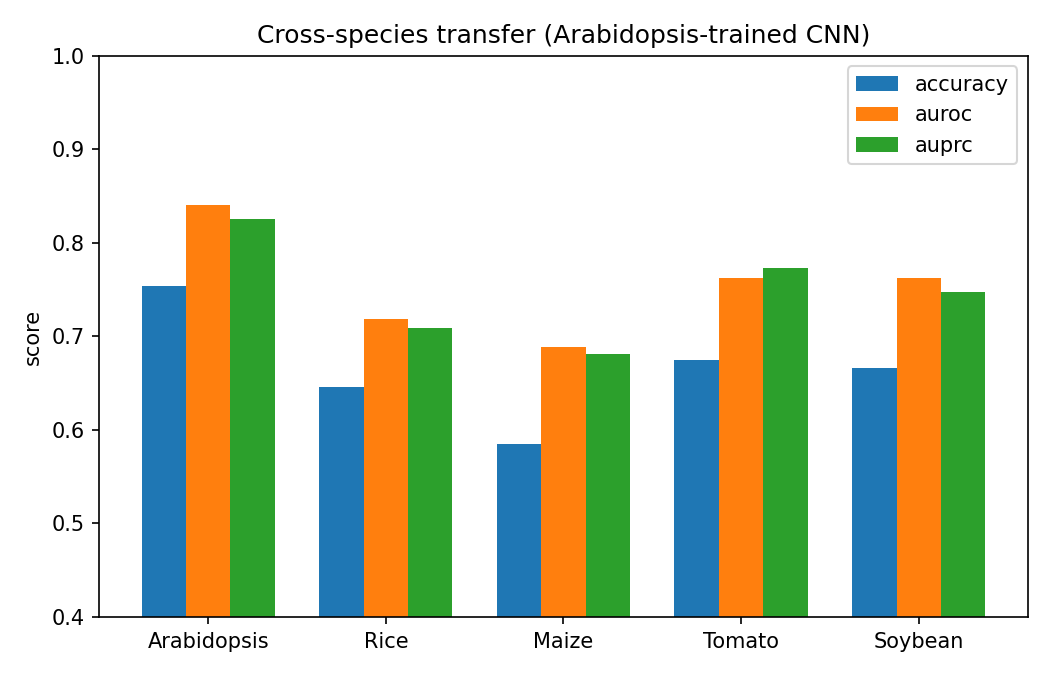
\includegraphics[width=0.7\textwidth]{fig6_cross_species.png}
\caption{Cross-species transfer of the Arabidopsis-trained CNN to four crop species plus the Arabidopsis reference (AUROC/accuracy/AUPRC on each species' test set).}
\label{fig:cross}
\end{figure}

% ============ 4. Discussion ============
\subsection{Cis-regulatory variant effect prediction}
Using the trained CNN, we scored 27{,}662 natural single-nucleotide variants mapping to gene flanking regions (from the Ensembl Plants Arabidopsis variation VCF). Variant effect magnitude ($|\Delta|$ predicted probability) differed strongly across regions: UTR variants—where the model assigns highest importance—showed significantly larger effects than terminator variants (median $|\Delta|$ 0.0017 vs.\ 0.0006; Mann--Whitney $p = 4.3\times10^{-98}$; Figure~\ref{fig:variant}). This shows the model's variant-effect scores concentrate where its attribution identifies regulatory importance, a self-consistent readout of cis-regulatory variation.

\begin{figure}[htbp]
\centering
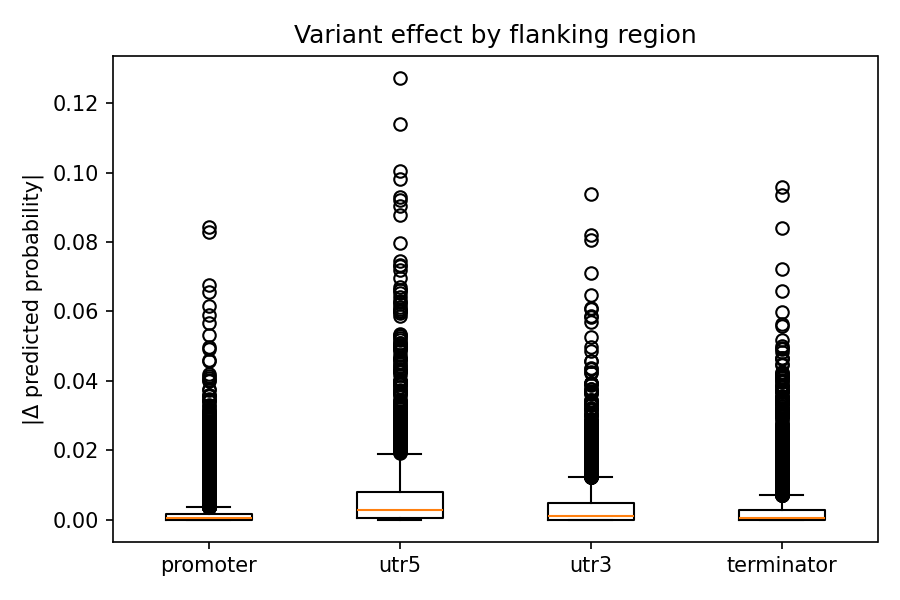
\includegraphics[width=0.72\textwidth]{fig5_region_validation.png}
\caption{Cis-regulatory variant effect magnitude by flanking region (boxplots of $|\Delta|$ predicted probability).}
\label{fig:variant}
\end{figure}

\section{Discussion}
\textbf{A unified reference for architecture choice.} Our head-to-head comparison quantifies, on a shared plant benchmark, the performance gain of a DNA foundation model over a conventional CNN. The $\sim$0.1 AUROC gain is large enough to matter for genome-scale expression annotation, and it is obtained at a modest cost because LoRA confines training to 1.6\% of parameters. These numbers give practitioners a concrete performance--cost reference for plant regulatory genomics.

\textbf{What the models learn.} Attribution-based regional analysis shows that the strongest expression signal lies in UTRs, consistent with their role in transcript stability and translation, and that the discovered motifs extend motif databases with expression-linked candidate CREs.

\textbf{Limitations.} The AgroNT model was fine-tuned for a limited number of epochs; additional training would likely further extend the reported gap. The CNN baseline is a single, moderately sized architecture. DeepLift motif discovery was performed on the CNN, with AgroNT region importance assessed only by perturbation; token-level attribution of the foundation model remains a natural next step. Variant-effect analysis uses regional enrichment rather than genome-wide eQTL association.

% ============ 5. Conclusions ============
\section{Conclusions}
We provide a unified, reproducible benchmark showing that a plant DNA foundation model (AgroNT) substantially outperforms a 1D-CNN baseline for sequence-based gene expression prediction in \emph{Arabidopsis thaliana}, and that the learned regulatory signal is concentrated in UTRs and transfers across species. These results establish a reference point for architecture selection in plant regulatory genomics and a practical pipeline for interpretable, cross-species expression modeling.

% ============ Back matter ============
\section*{Data and Code Availability}
Code is available at the project repository (DOI to be assigned). All data are public: PGB \cite{pgb2024}, TAIR10/Araport11, JASPAR.

\section*{References}
\begin{thebibliography}{99}
\small
\setlength{\itemsep}{2pt}

\bibitem{peleke2024}
Peleke, F.F.; Zumkeller, S.M.; G\"ultas, M.; Schmitt, A.; Szyma\'nski, J. Deep learning the cis-regulatory code for gene expression in selected model plants. \emph{Nat.\ Commun.} \textbf{2024}, \emph{15}, 3488.

\bibitem{mendoza2024}
Mendoza-Revilla, J.; Trop, E.; Gonzalez, L.; et al. A foundational large language model for edible plant genomes. \emph{Commun.\ Biol.} \textbf{2024}, \emph{7}, 835.

\bibitem{marand2023}
Marand, A.P.; Eveland, A.L.; Kaufmann, K.; Springer, N.M. cis-Regulatory elements in plant development, adaptation, and evolution. \emph{Annu.\ Rev.\ Plant Biol.} \textbf{2023}, \emph{74}, 111--137.

\bibitem{hu2023}
Hu, X.; Fernie, A.R.; Yan, J. Deep learning in regulatory genomics: from identification to design. \emph{Curr.\ Opin.\ Biotechnol.} \textbf{2023}, \emph{79}, 102887.

\bibitem{zhou2015}
Zhou, J.; Troyanskaya, O.G. Predicting effects of noncoding variants with deep learning--based sequence model. \emph{Nat.\ Methods} \textbf{2015}, \emph{12}, 931--934.

\bibitem{shrikumar2017}
Shrikumar, A.; Greenside, P.; Kundaje, A. Learning important features through propagating activation differences. In \emph{Proceedings of the 34th International Conference on Machine Learning}, PMLR 70, 2017; pp.\ 3145--3153.

\bibitem{pgb2024}
InstaDeepAI. Plants Genomic Benchmark (PGB). Hugging Face. DOI 10.57967/hf/2464.

\end{thebibliography}

\end{document}
